\section{Introduction}  

In this section we will briefly introduce the aim of this project and the algorithm that we studied and implemented in a parallel fashion.
The algorithm is the Gauss-Newton algorithm for non linear least square interpolation.
In this particular case we studied an implementation of the algorithm for three dimensional interpolation of images representing gaussian beams.
The sequential version of the algorithm was developed in summer 2009 for interpolation of images of laser beams captured by digital cameras. 
By interpolation it is possible to monitor the output of a high definition camera with a precision down to micrometers, this operation requires lots of computation nonetheless.
This constitute the main reason for a parallel version of the program.

\subsection{Experimental Setup}

In this section we will briefly illustrate the environment where the algorithm is used and the main purpose for its development.
Laser beams are used to monitor the position and orientation of suspended mirrors used in the LIGO interferometer AGGIUNGI BIB. 
The beam is pointed towards the mirror with a 45 degree angle and reflected on the screen of a high resolution digital camera.
Tilting of the mirror will produce a movement in the position of the laser beam while distortion of the surface of the mirror will produce a change in focus (size) of the beam.
Using then multiple cameras is possible to have a complete three dimensional displacement of the mirror in real time.
In order to do so position and size of the beam should be monitored with high precision. 
As said before the best way to do so is to interpolate the profile of the captured image of the laser beam which, in normal operative conditions, have a perfect gaussian shape.
Since the output of the camera is used for adjustments on remote controlled machinery it is important to have both a high throughput in terms of number of images elaborated and high precision of the interpolation itself.
In our opinion this was a nice real life case for our project.
Now let's analyse the algorithm used for interpolation.

\subsection{Algorithm}

The algorithm is the well known Gauss-Newton algorithm for non linear least square problems.
As the name says this algorithm does not perform perfect interpolation but tries to reduce as most the square error between the interpolated function and the real data.
Linear methods as polynomial interpolation can be solved in a single step operating on every point (pixel) only once, non linear methods are iterative and so tends to converge after a certain number of steps.
The pseudo code of the algorithm is shown in Figure \ref{code:gauss}.

\begin{figure}[h]
\begin{center} 
\begin{minipage}[c]{.85\textwidth} 
\centering 
\begin{pseudo}{}{gauss}
unsigned char $image[num\_pixel]$;
double $parameters$[8], $delta\_vector[8]$, $diff\_vector[num\_pixel]$, $gradient\_matrix[num\_pixel][8]$, $gradient\_result[8][8]$, $gradient\_vector[8]$;
double $error$, $threshold$;

get_image($image$);
get_parameters($parameters$);

while ($error$ > $threshold$ ) {
    for($i$ = 0; $i$ < $num\_pixel$; $i$ ++){
	
          $diff\_vector$[$i$] = $image$[$i$] - evaluateGaussian($parameters$,$i$); 
          $gradient\_matrix[i][:]$ = computeGradients($i$,$parameters$);
	      
    }
    $gradient\_result$ = $gradient\_matrix^T$ * $gradient\_matrix$;
    $gradient\_vector$ = $gradient\_matrix^T$ * $diff\_vector$;
    $delta\_vector[:]$ = LU_solve ($gradient\_result$ , $gradient\_vector$);
    $parameters[:]$ += $delta\_vector[:]$;
    $error$ = compute_square_error($image$, $parameters$);
}
return $parameters$;

\end{pseudo}
\end{minipage} 
\end{center} 
\label{code:gauss}
\caption{Pseudo code of Gauss-Newton algorithm}
\end{figure}

It is important to point out some interesting facts.
Ideally the algorithm could loop for an infinite number of iterations but since we are dealing with finite arithmetic the algorithm will surely converge after a finite number of steps.
Consider that, since we are monitoring a slowly changing environment, one iteration is sufficient in order to converge to a result with desired precision. 
Unfortunately cameras are in the Caltech facility so we also had to develop a simulator for the camera itself.

\begin{figure}[h]
\centering
\subfigure[]{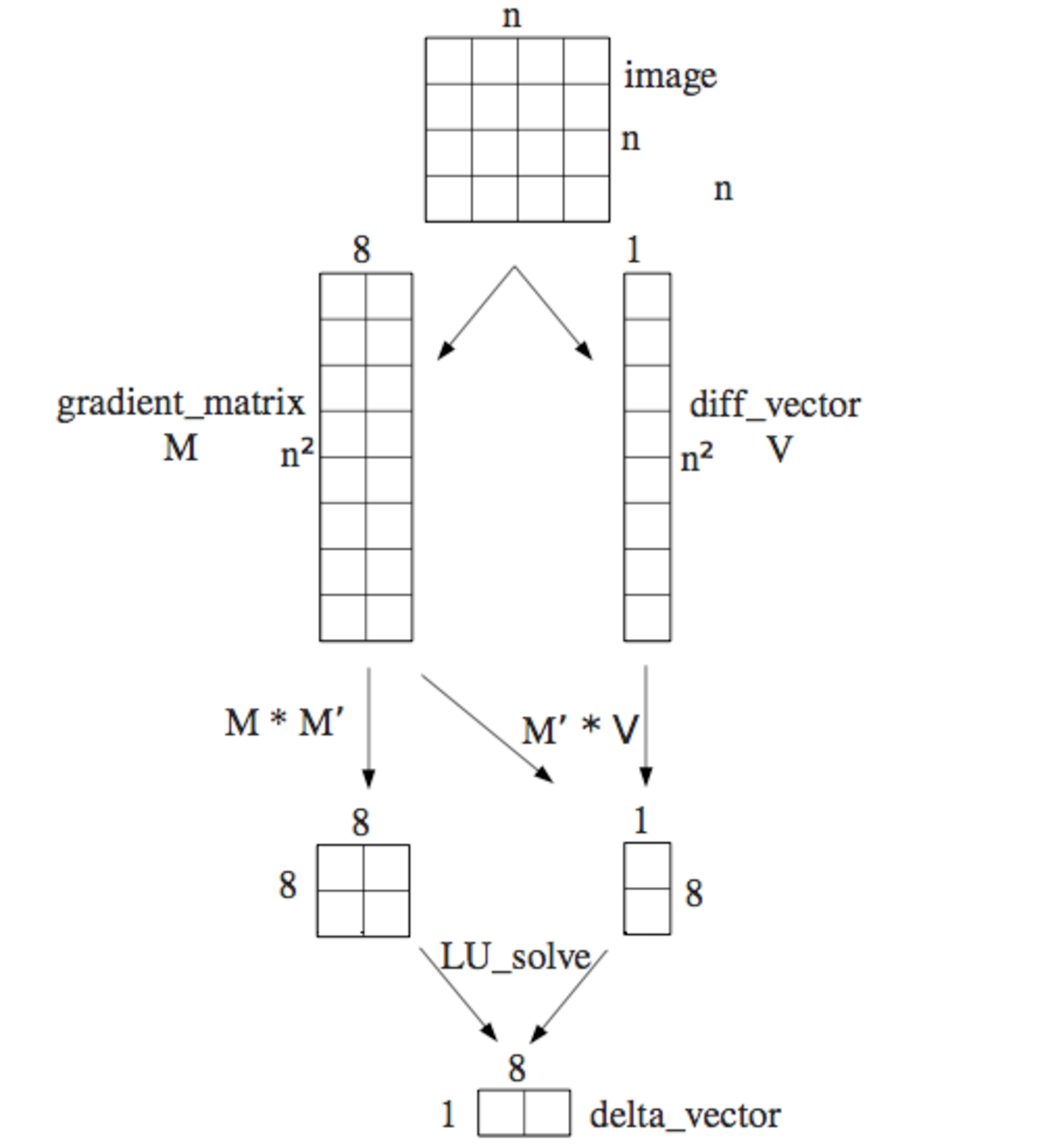
\includegraphics[width=115mm,height=130mm]{./algorithm}
\label{steps}}
\caption{Gauss-Newton algorithm steps}
\end{figure}
\subsection{Parallel Schemes}

Now let's get more into details of the parallelization.
As a first thing we have to model the parallel computation using a structured parallel programming scheme. 
We know that there is an (ideal) infinite stream of images and the computation is a pure function, hence a way to parallelize this program can be the farm approach: we can replicate the algorithm in each worker node with a cost model that we will introduce soon. 
For this scheme is not necessary to know the internal structure of the algorithm, but if we analyse it, we recognize some interesting aspects.

Following the pseudo code in Figure 1 we have:
\begin{enumerate}
\item the construction of the \textit{diff\_vector} and the \textit{gradient\_matrix} starting from the image.
\item the multiplication between the \textit{gradient\_matrix} and its own transposed matrix and  the multiplication between the transposed matrix and the \textit{diff\_vector}.
\item the LU\_solve operation.
\item the sum of the vector \textit{parameter} with \textit{delta\_vector}.
\end{enumerate}

It is clear that only computation in $1$ and $2$ is relevant since the linear system resolution is performed with a really small data size.
We can also notice that the operation performed in such steps are independent for every pixel.
This suggests a data parallel scheme which involve replication of functions and partioning of the data.
This means that there is no need of communications of values between different partitions of the matrix but it is necessary to communicate the partial results calculated by every worker and sum them and to obtain the $8$x$8\ gradient\_matrix$ and the vector $gradient\_vector$. 
Finally, we notice that the last point must be executed only after the calculations above and they take a negligible time respect than the previous operations.

This situation suggests a parallelism scheme in which the data can be partitioned between different modules for computing the first two points and a reduce operation is performed in order to execute the last two steps on single node. 
This is the well known map reduce scheme.

At this point we chose to realize both a farm and data parallel scheme. We will further discuss their cost model in the next section.